\documentclass[a4paper,utf8]{article}
\usepackage[heading,fancyhdr]{ctex}
\usepackage{amsmath,amssymb,geometry,lastpage,ulem}
\usepackage{array,tabularx,graphicx,floatrow}
\geometry{
    top=25.4mm, 
    left=30mm, 
    right=30mm, 
    bottom=35mm,
    headsep=5.9mm,
}
\ctexset{
    section = {format+=\raggedright}
}
\newcommand{\expinfo}[5]{
    {\zihao{-3}\bfseries\songti
    实验名称:\uline{\hfill\mbox{#1}\hfill} \\[2.9mm]
    学\quad 号:\uline{\makebox[25mm]{#2}}\hfill
    姓\quad 名:\uline{\makebox[25mm]{#3}}\hfill
    班\quad 级:\uline{\makebox[25mm]{#4}} \\[2.9mm]
    合作者:\uline{\makebox[25mm]{无}}\enspace~
    桌\quad号:\uline{\makebox[25mm]{}}\hfill\mbox{}\\[2.9mm]
    指导教师:\uline{\makebox[30mm]{#5}}\hfill\mbox{} \\[2.9mm]
    实验日期:\uline{\makebox[30mm]{}}\hfill\mbox{} \\[58.7mm]
    }
}%\expinfo{实验名称}{学号}{姓名}{班级}{指导教师}
\pagestyle{fancy}
\fancyhf{} \fancyhead[C]{材料科学基础实验} \fancyfoot[C]{\thepage~/~\pageref{LastPage}}
\begin{document}
\begin{center}
    {\mbox{}\\[7em]\zihao{2}\bfseries\songti%
    材料科学基础实验报告}\\[34mm]
    \expinfo{实验四 碳钢淬火、回火后的组织观察与硬度分析}{22301070}{杨雨燃}{22材物}{杨玉华}
    {\zihao{4}\bfseries\songti
    实验考核\\[3mm]
    \extrarowheight=3mm
    \begin{tabularx}{150mm}{|X|X|X|X|X|}\hline
        \hfil 项目 \hfil  & \hfil 实验预习 \hfil & \hfil 实验过程 \hfil & \hfil 分析与讨论 \hfil & \hfil 总评 \hfil \\[3mm] \hline
        \hfil 评价 \hfil &  &  &  &  \\[3mm] \hline
    \end{tabularx}
    }
\end{center}
\newpage
\section*{【实验目的】}
    \begin{enumerate}
        \item 了解碳钢的淬火、回火过程。
        \item 观察和研究碳钢经不同淬火、回火处理后显微组织的特点,分析冷却条件、淬火温度及回火条件对其组织形态与硬度的影响,并了解淬火、回火的应用领域。
    \end{enumerate}   
\section*{【实验原理】}%简单描述,含必要的公式和附图;

\textbf{(一) 淬火}

淬火是将钢奥氏体化后以大于临界冷却速度的速度进行冷却,获得马氏体或下贝氏体组织的热处理工艺。其主要目的是为了获得马氏体,提高试样的硬度和强度。

1、淬火温度的选择:
\begin{center}
    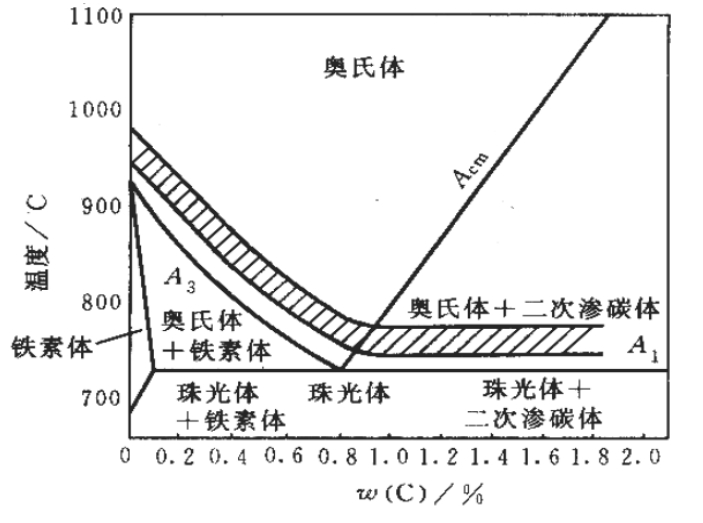
\includegraphics[width=200pt]{1.png}
\end{center}

2、保温时间:保温的目的是使钢件热透,使奥氏体充分转变为均匀化。计算公式为:
\begin{center}
    τ = $\alpha$KD
\end{center}
 
式中,$\alpha$为加热系数;K为装炉系数;D为有效尺寸,mm。

3、淬火冷却介质:钢在加热获得奥氏体后要选用适当的冷却介质进行冷却,获得马氏体组织。常用的冷却介质有油、水、盐水、碱水等,其冷却能力依次增加,但是这些冷却介质都存在不同的缺点。

4、淬火后的组织:

低碳钢淬火后能观察到一束束接近相互平行的细条状马氏体群;

中碳钢淬火将得到细针
状马氏体和板条状马氏体的混合组织;

高碳钢,如共析钢和过共析钢在等温淬火后可得到贝氏体组织;亚共析钢淬火后能观察到板条状或针的状马氏体组织,共析钢和过共析钢在
淬火后亦得到马氏体组织。

\begin{center}
    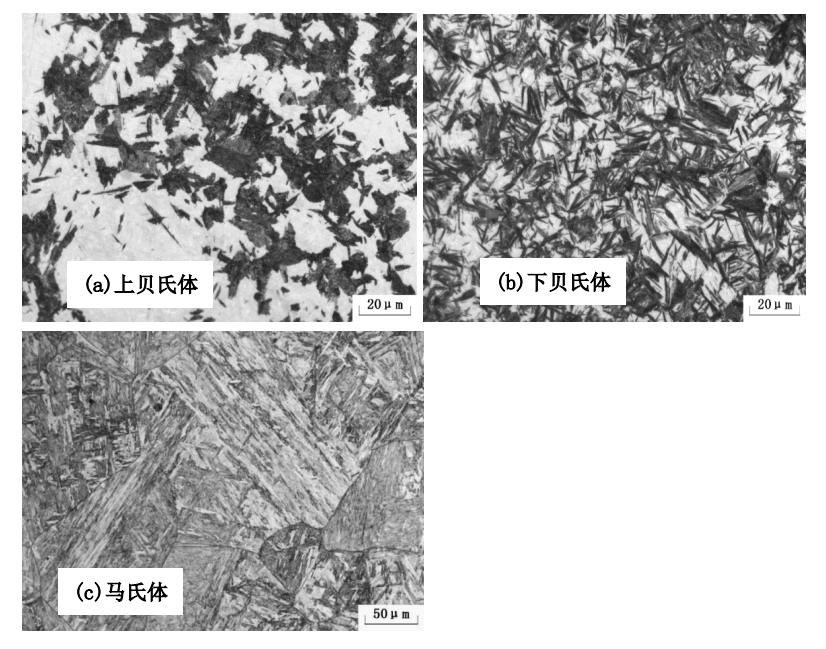
\includegraphics[width=300pt]{6.png}
\end{center}

\textbf{(二) 回火}

回火是将经过淬火的试样加热到临界点$A_1$ 以下的适当温度,保持一定时间后,采用适当的冷却方式进行冷却的热处理工艺。主要是消除内应力,获得所要求的力学性能以提高尺寸和稳定性。

① 回火马氏体:
低温回火后,颜色要比淬火马氏体深些,呈暗黑色的针状组织。 具有高的强度和硬度,同时韧性和塑性也较淬火马氏体有明显改善。

② 回火屈氏体:
中温回火后,在铁素体基体上弥散分布着微小粒状的渗碳体组织,渗碳体则呈细小的颗粒状,在光学显微镜下呈暗黑色不易分辨清楚。具有较好的强度和硬度,以及非常高的弹性性能。

③ 回火索氏体:
高温回火后,由颗粒状渗碳体和多边形的铁素体组成的组织。具有强度、韧性和塑性较好的综合机械性能。

\begin{center}
    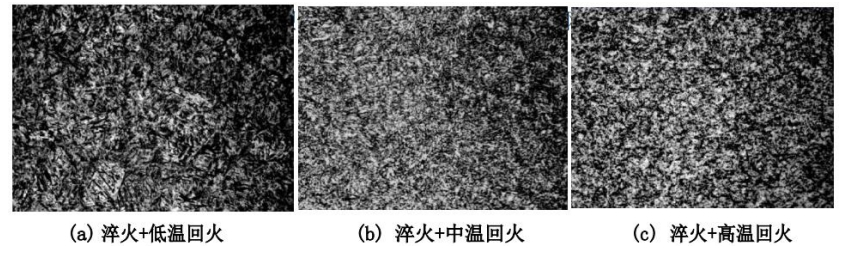
\includegraphics[width=400pt]{2.png}
\end{center}

\section*{【实验仪器】}%规格及参数
箱式电阻加热炉,洛氏硬度计,砂纸,抛光机,金相显微镜。热处理试样:
45钢及T12钢。
\section*{【实验过程】}%简述主要过程和实验内容
1、4人一组,45钢(2个)、T8(1个)及T12钢(1个),(对应下表中相应的热处理工艺方法)

\begin{center}
    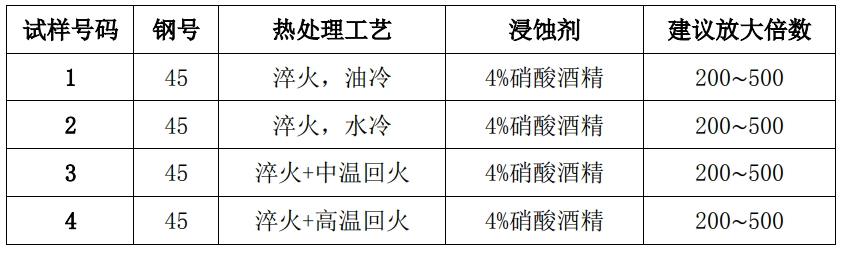
\includegraphics[width=350pt]{3.png}
\end{center}

2、制定热处理工艺参数,可参考以下工艺参数。τ = $\alpha$KD


(1. 45 钢淬火工艺:加热温度为 $860 \pm 10$℃,根据试样有效尺寸计算保温时间,保温后用长柄铁钳夹出放入\textbf{淬火油}中冷却。

(2. 45 钢淬火工艺:加热温度为 $860 \pm 10$℃,根据试样有效尺寸计算保温时间,保温后用长柄铁钳夹出放入\textbf{水}中进行冷却。

(3. 45 钢淬水+中温回火工艺:加热温度为 $860 \pm 10$℃,根据试样有效尺寸计算保温时间,保温后出炉进行水淬。随后放入炉中加热至 400℃,保温 1 个小时后出炉空冷。

(4. 45 钢淬水+高温回火工艺:加热温度为 $860 \pm 10$℃,根据试样有效尺寸计算保温时间,保温后出炉进行水淬。随后放入炉中加热至 600℃,保温 1 个小时后出炉空冷。


3、利用硬度计对所有热处理后的试样进行硬度测试,每个试样至少三个试验点,再取一个平均值,分析热处理工艺对其硬度的影响。按照下表选用硬度计。(硬度测试须在金相磨制观
察前完成)

\begin{center}
    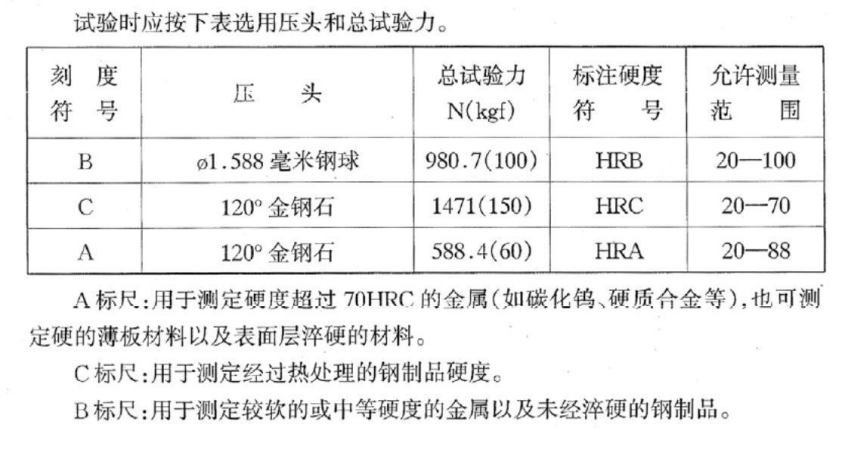
\includegraphics[width=350pt]{4.png}
\end{center}


4、根据拟定的热处理工艺对试样进行相应的热处理工艺处理,然后利用金相砂
纸对热处理后的试样进行磨制、抛光,并用4\%的硝酸酒精进行腐蚀制得金相试样。
利用金相显微镜对其进行显微组织观察,分析热处理工艺对其组织的影响。

5、实验结束后,汇总各小组实验数据,根据实验数据分析冷却方法及回火温度对碳钢性能(硬度)的影响,画出回火温度同硬度的关系曲线,并阐明硬度变化的原因。
\section*{【实验数据及处理】}

测试硬度的硬度计表盘最小分度均为0.1HRB(HRC)

因而,我们可以依照公式得到其硬度的不确定度。如下表。
公式如下:(X为硬度,$\bar{X} $为硬度的平均值)
\begin{center}\zihao{4}
    $ S = \frac{\Sigma |X - \bar{X}| }{3} $
\end{center}


\begin{table}[!ht]\centering
    \caption{不同热处理试样的硬度}
    \extrarowheight=11pt
    \begin{tabularx}{\textwidth}{|c|X|X|X|X|X|}\hline
        材料及热处理状态 & \multicolumn{3}{c|}{测得硬度数据(HRC)} & \hfil 平均值 \hfil &不确定度 \\[10pt] \hline
        45 钢油淬 & 27.1 & 28.0 & 25.9 & 27 &0.7\\[10pt] \hline
        45 钢水淬 & 62.4 & 62.3 & 61.0 & 61.9 &0.6\\[10pt] \hline
        45 钢水淬,200摄氏度回火前 & 61.9 & 57.5 &60.0  & 60.1 &1.5\\[10pt] \hline
        45 钢水淬,200摄氏度回火后 & 56.4 & 56.0 &56.6  & 56.3 &0.4\\[10pt] \hline
        45 钢水淬,400摄氏度回火前 & 61.2 & 61.8 &62.1  &61.7 &0.3\\[10pt] \hline
        45 钢水淬,400摄氏度回火后 & 40.2 & 41.2 &40.5  &40.6 &0.4\\[10pt] \hline
        45 钢水淬,600摄氏度回火前 & 57 & 59.5 &63.0  & 59.8 &2.1\\[10pt] \hline
        45 钢水淬,600摄氏度回火后 & 25 & 26.5 &23.0  & 24.8 &1.2\\[10pt] \hline
    \end{tabularx}
\end{table}

分析:

1.45钢油淬,相比45钢水淬硬度更低,这是因为油淬的降温速度更慢,相比水淬,其淬硬层更薄,同时微观结构中的片状马氏体更大,
导致其结构不够细密,力学性质不如水淬钢。

2.通过对比回火前后的硬度,我们可以发现,回火后硬度普遍下降了,其中,低温回火下降的最不明显,
中温回火硬度下降更多,高温回火下降最多,原因在于,回火时会引起残余奥氏体和马氏体的分解,导致其结构
不如先前强,不同的回火温度,其结构也有差异。

3.在不同回火温度下,硬度降低值不相同,600摄氏度回火组硬度最低,400摄氏度回火组硬度较低,200摄氏度回火组,硬度最高,
随着回火温度的提升,更多的残余奥氏体和马氏体参与分解,使得原淬火后的马氏体组织被破坏,硬度越小,该钢
获得更好的韧性。
\newpage
\section*{【实验图像记录】}

1).45钢油淬

\begin{figure}[!ht]
    \begin{floatrow}
        \ffigbox[60mm]{\caption{45钢油淬1}}{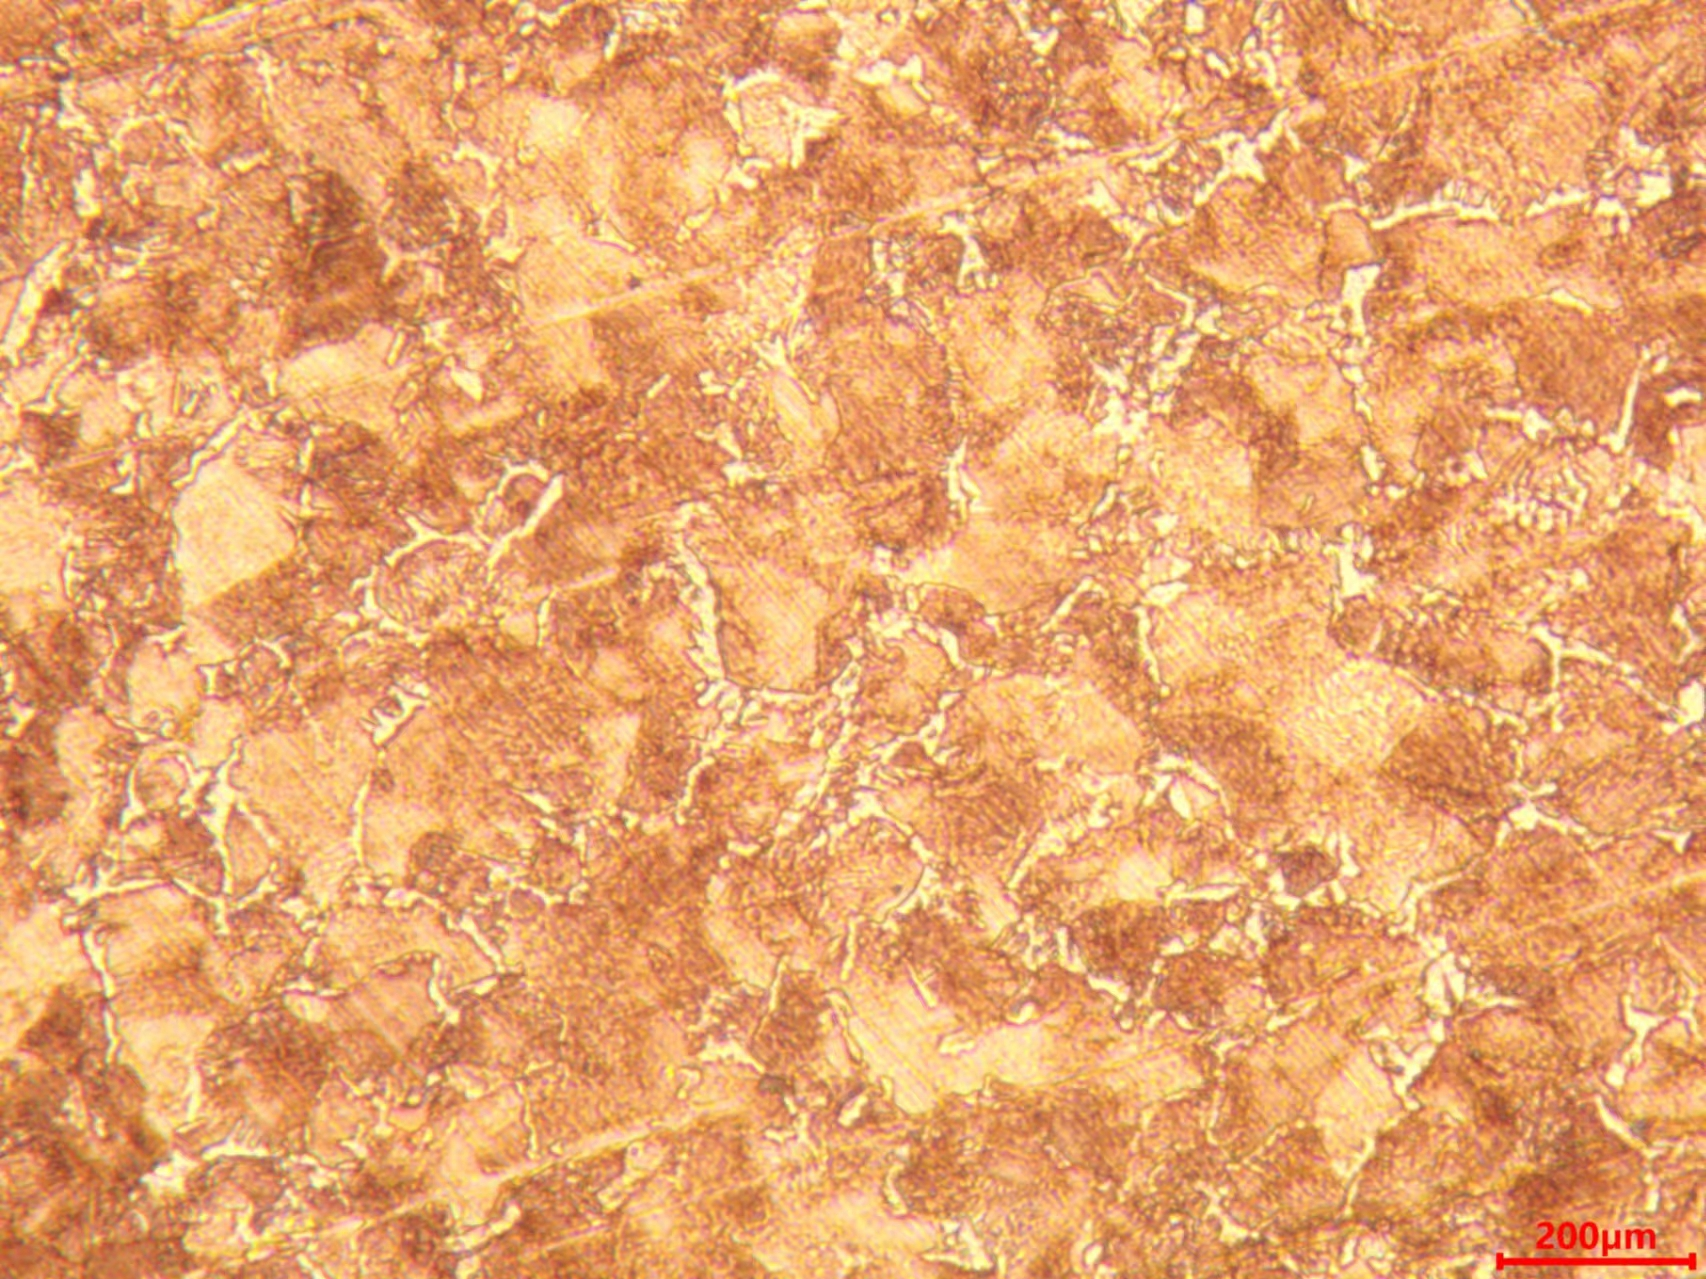
\includegraphics[width=60mm]{111.jpg}}
        \ffigbox[60mm]{\caption{45钢油淬2}}{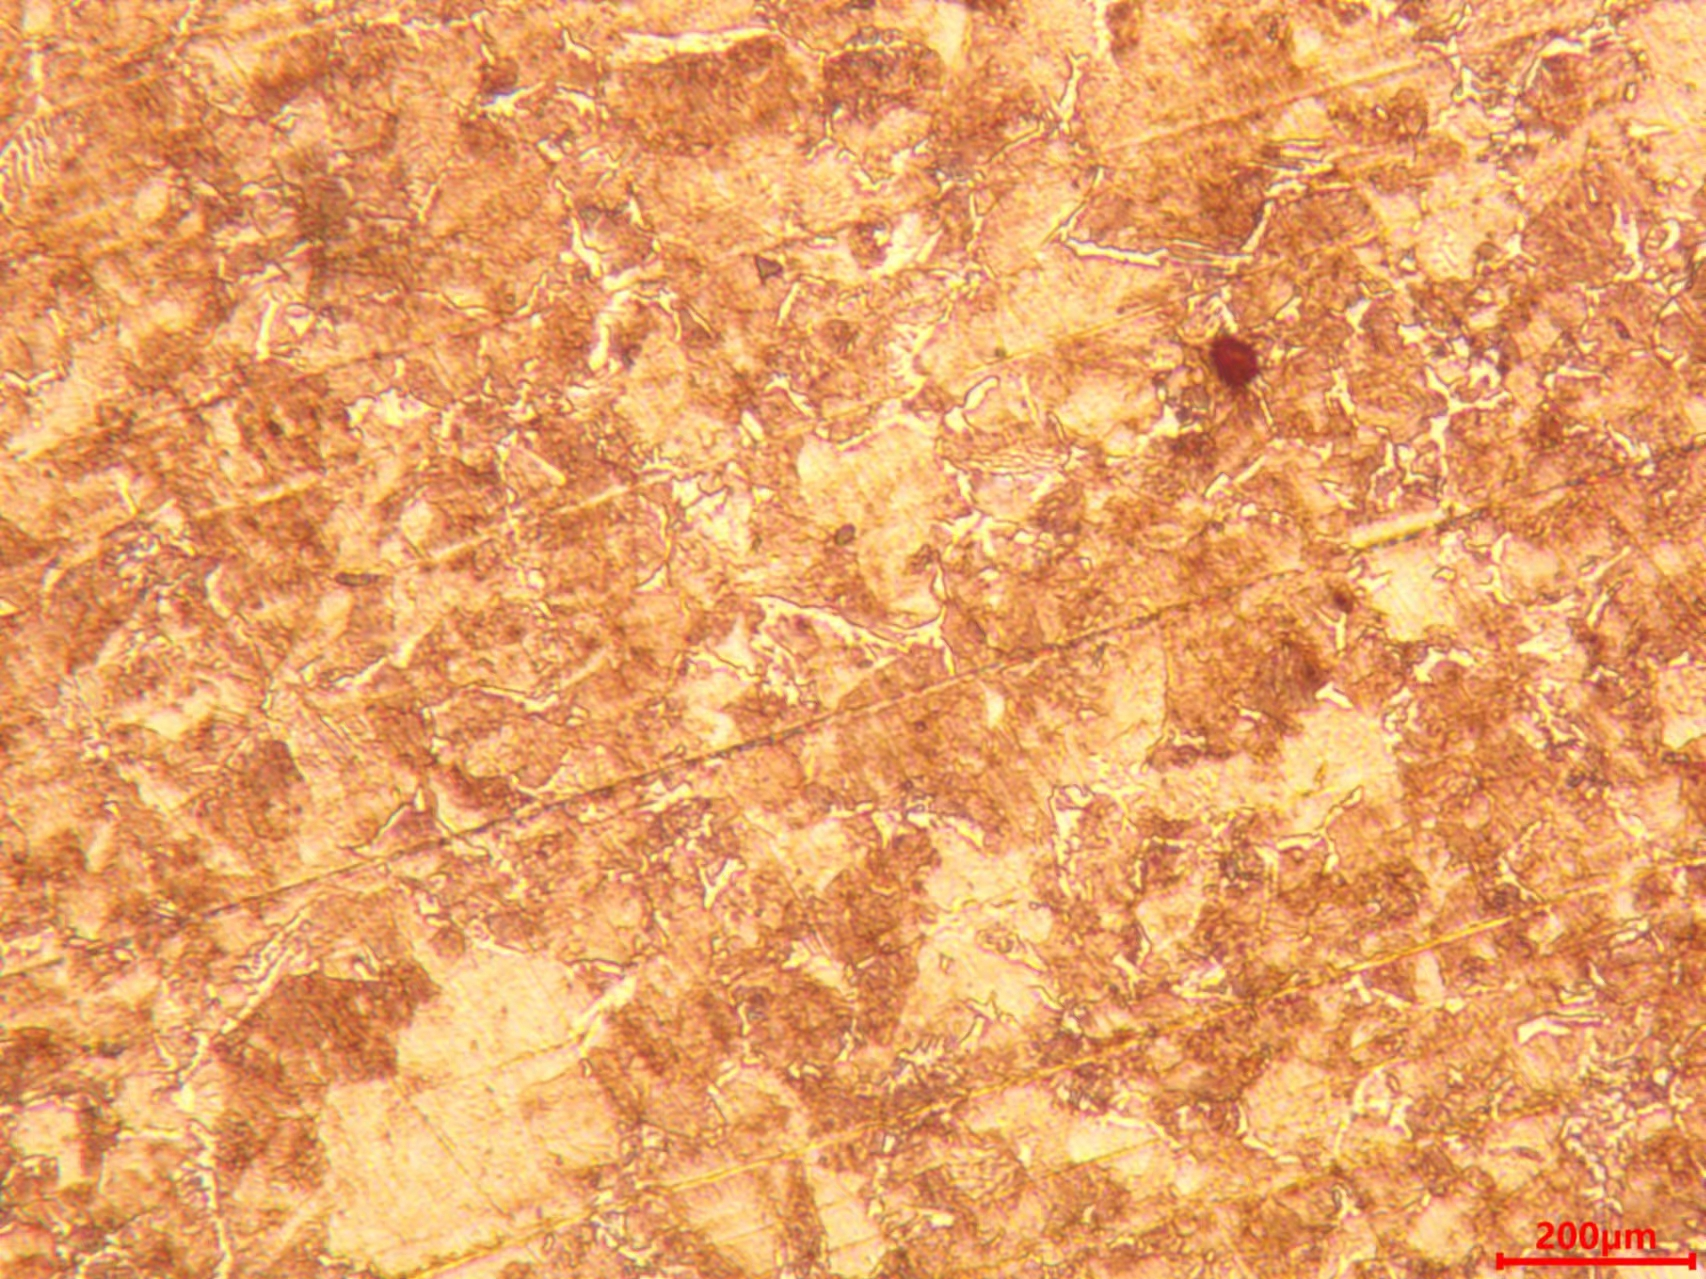
\includegraphics[width=60mm]{112.jpg}}
    \end{floatrow}

\end{figure}

分析:亚共析钢淬火后能观察
到板条状或针的状马氏体组织。

图中可以看出,暗的部分是片状的马氏体,理论上应该有针状的马氏体,但是由于油淬降温速度更慢
,其针状的马氏体更不明显,在显微镜下难以分辨。同时,本样品在显微镜下确实难以找到针状的马氏体,
制样也可能对此有影响。

2).45钢水淬

\begin{figure}[!ht]
    \begin{floatrow}
        \ffigbox[60mm]{\caption{45钢水淬1}}{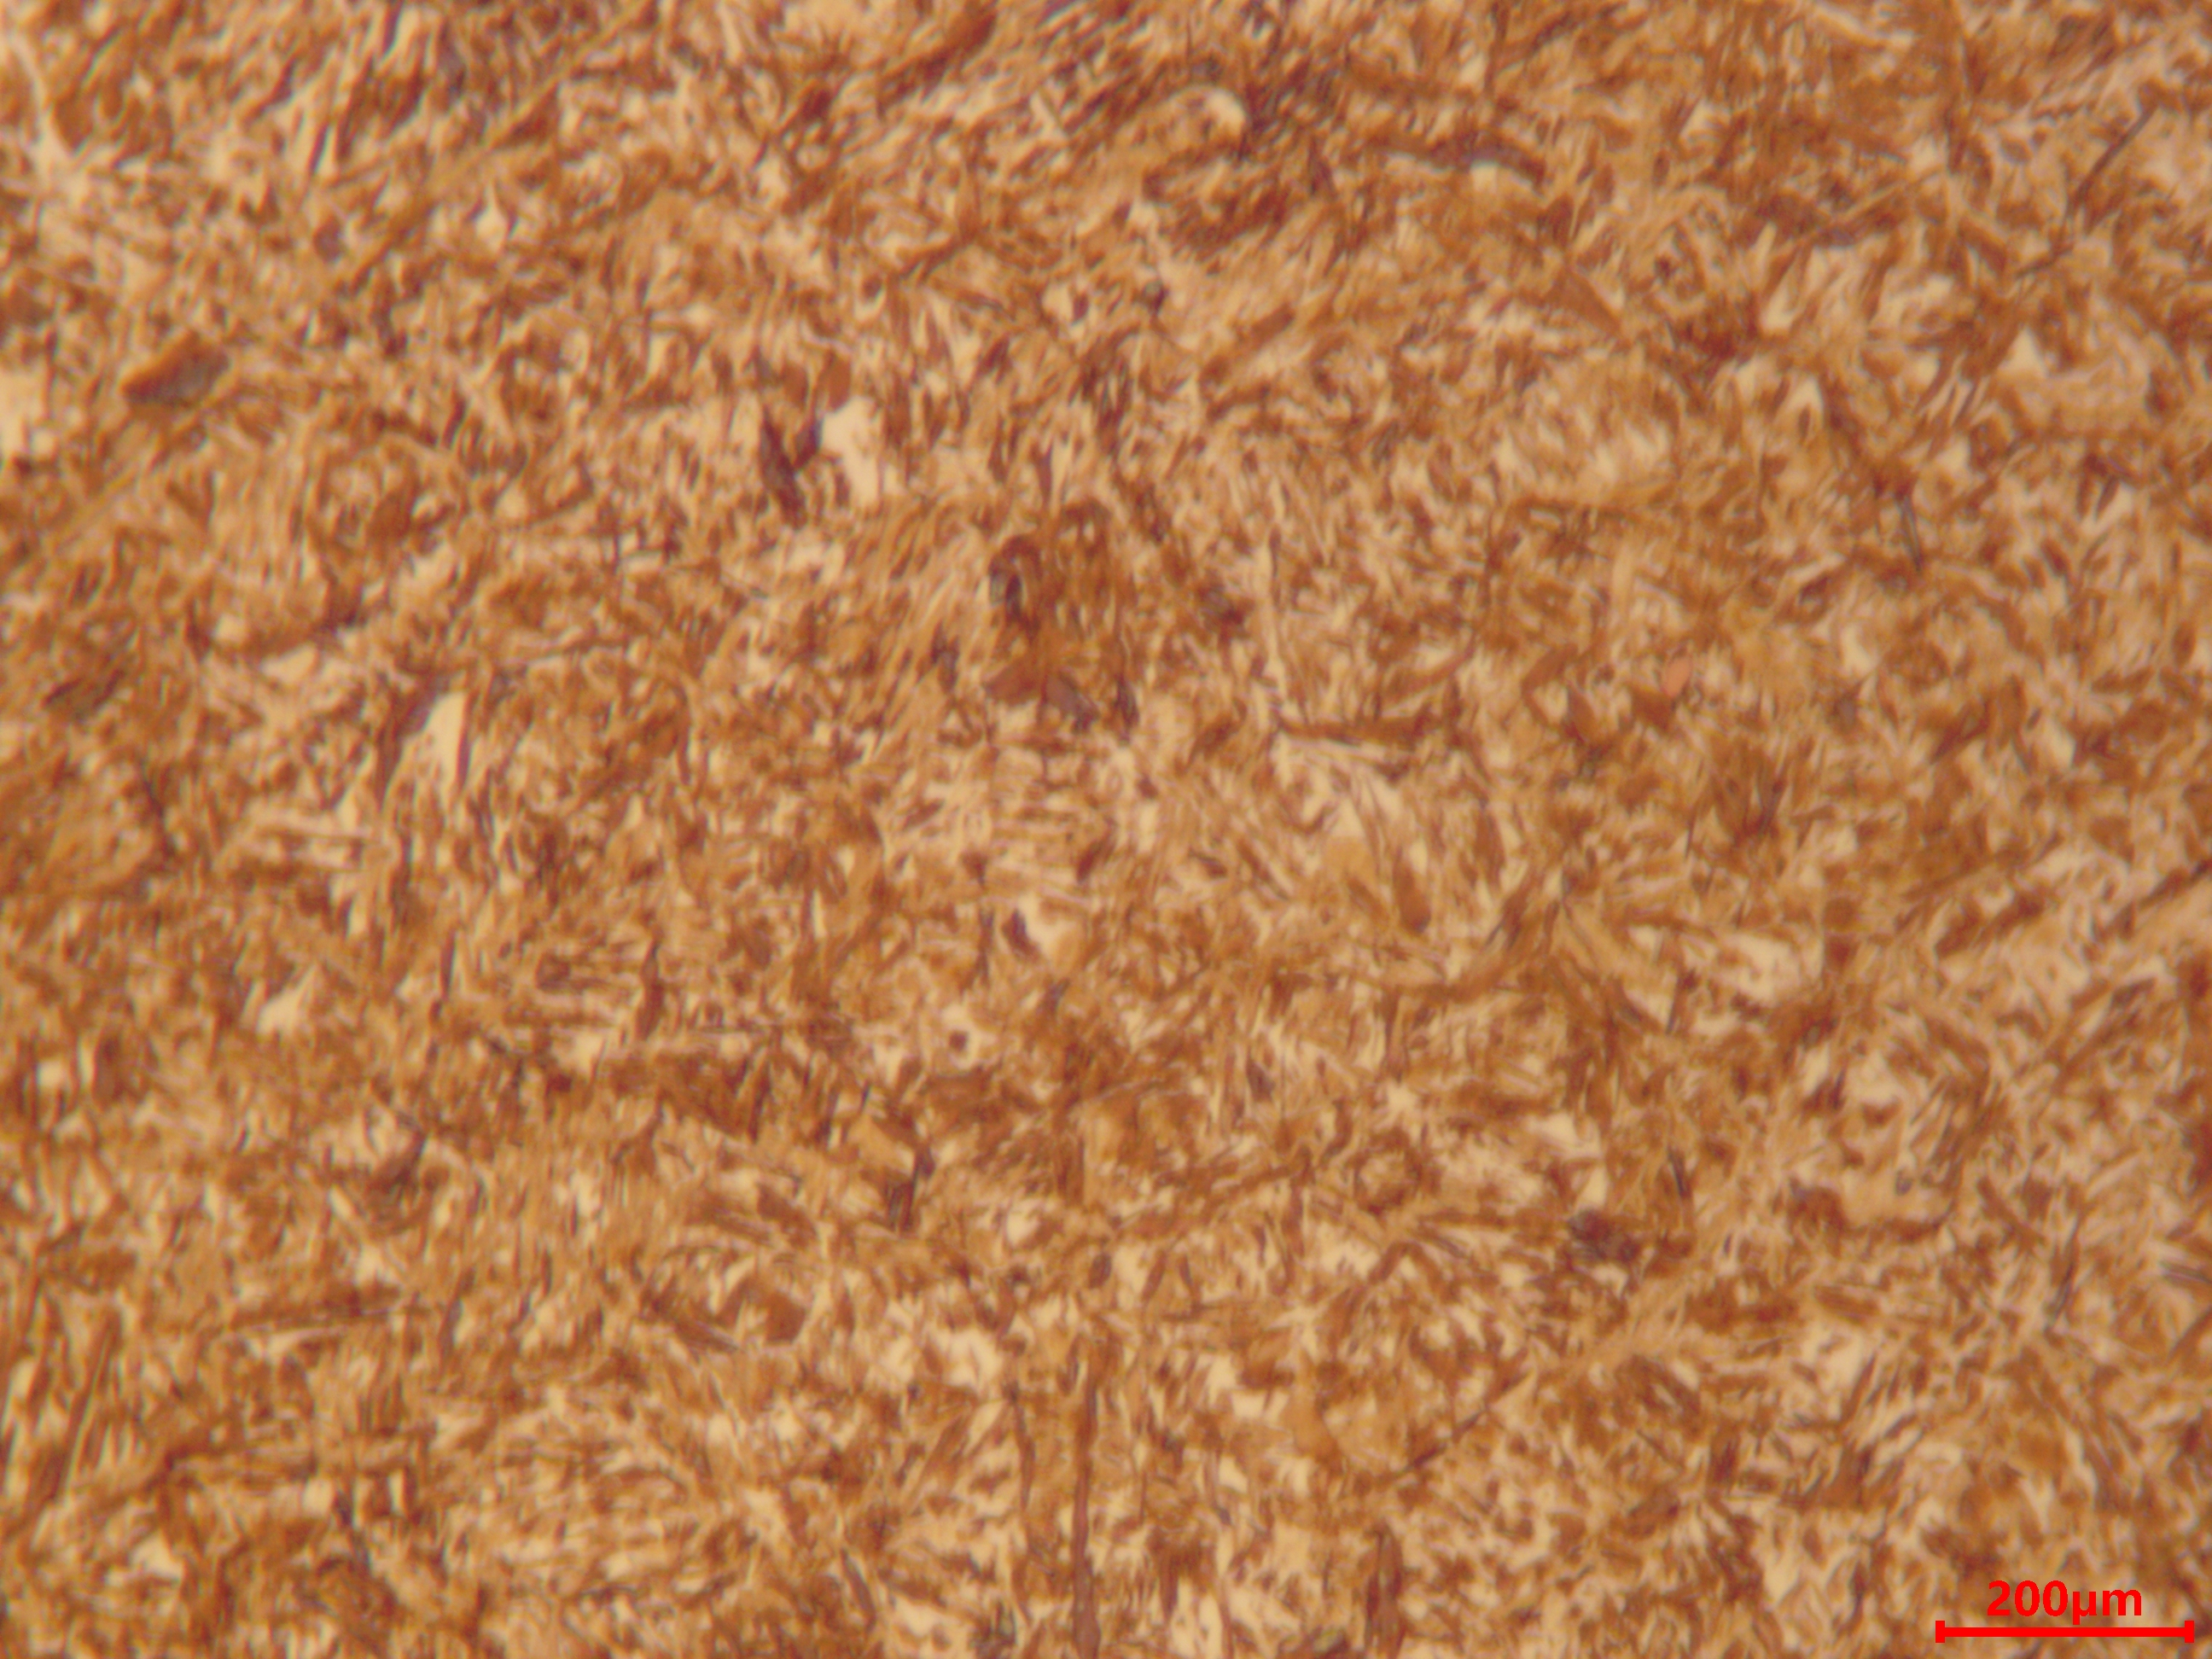
\includegraphics[width=60mm]{121.jpg}}
    \end{floatrow}

\end{figure}

分析:亚共析钢淬火后能观察
到板条状或针的状马氏体组织,我们可以观察到片状的马氏体以及针状的马氏体,由于水淬冷却更快,所以,
其结构更细小,针状的马氏体更多,马氏体看起来更加密集。

\newpage
3).45钢水淬,200摄氏度回火
\begin{figure}[!ht]
    \begin{floatrow}
        \ffigbox[60mm]{\caption{45钢水淬,200摄氏度回火}}{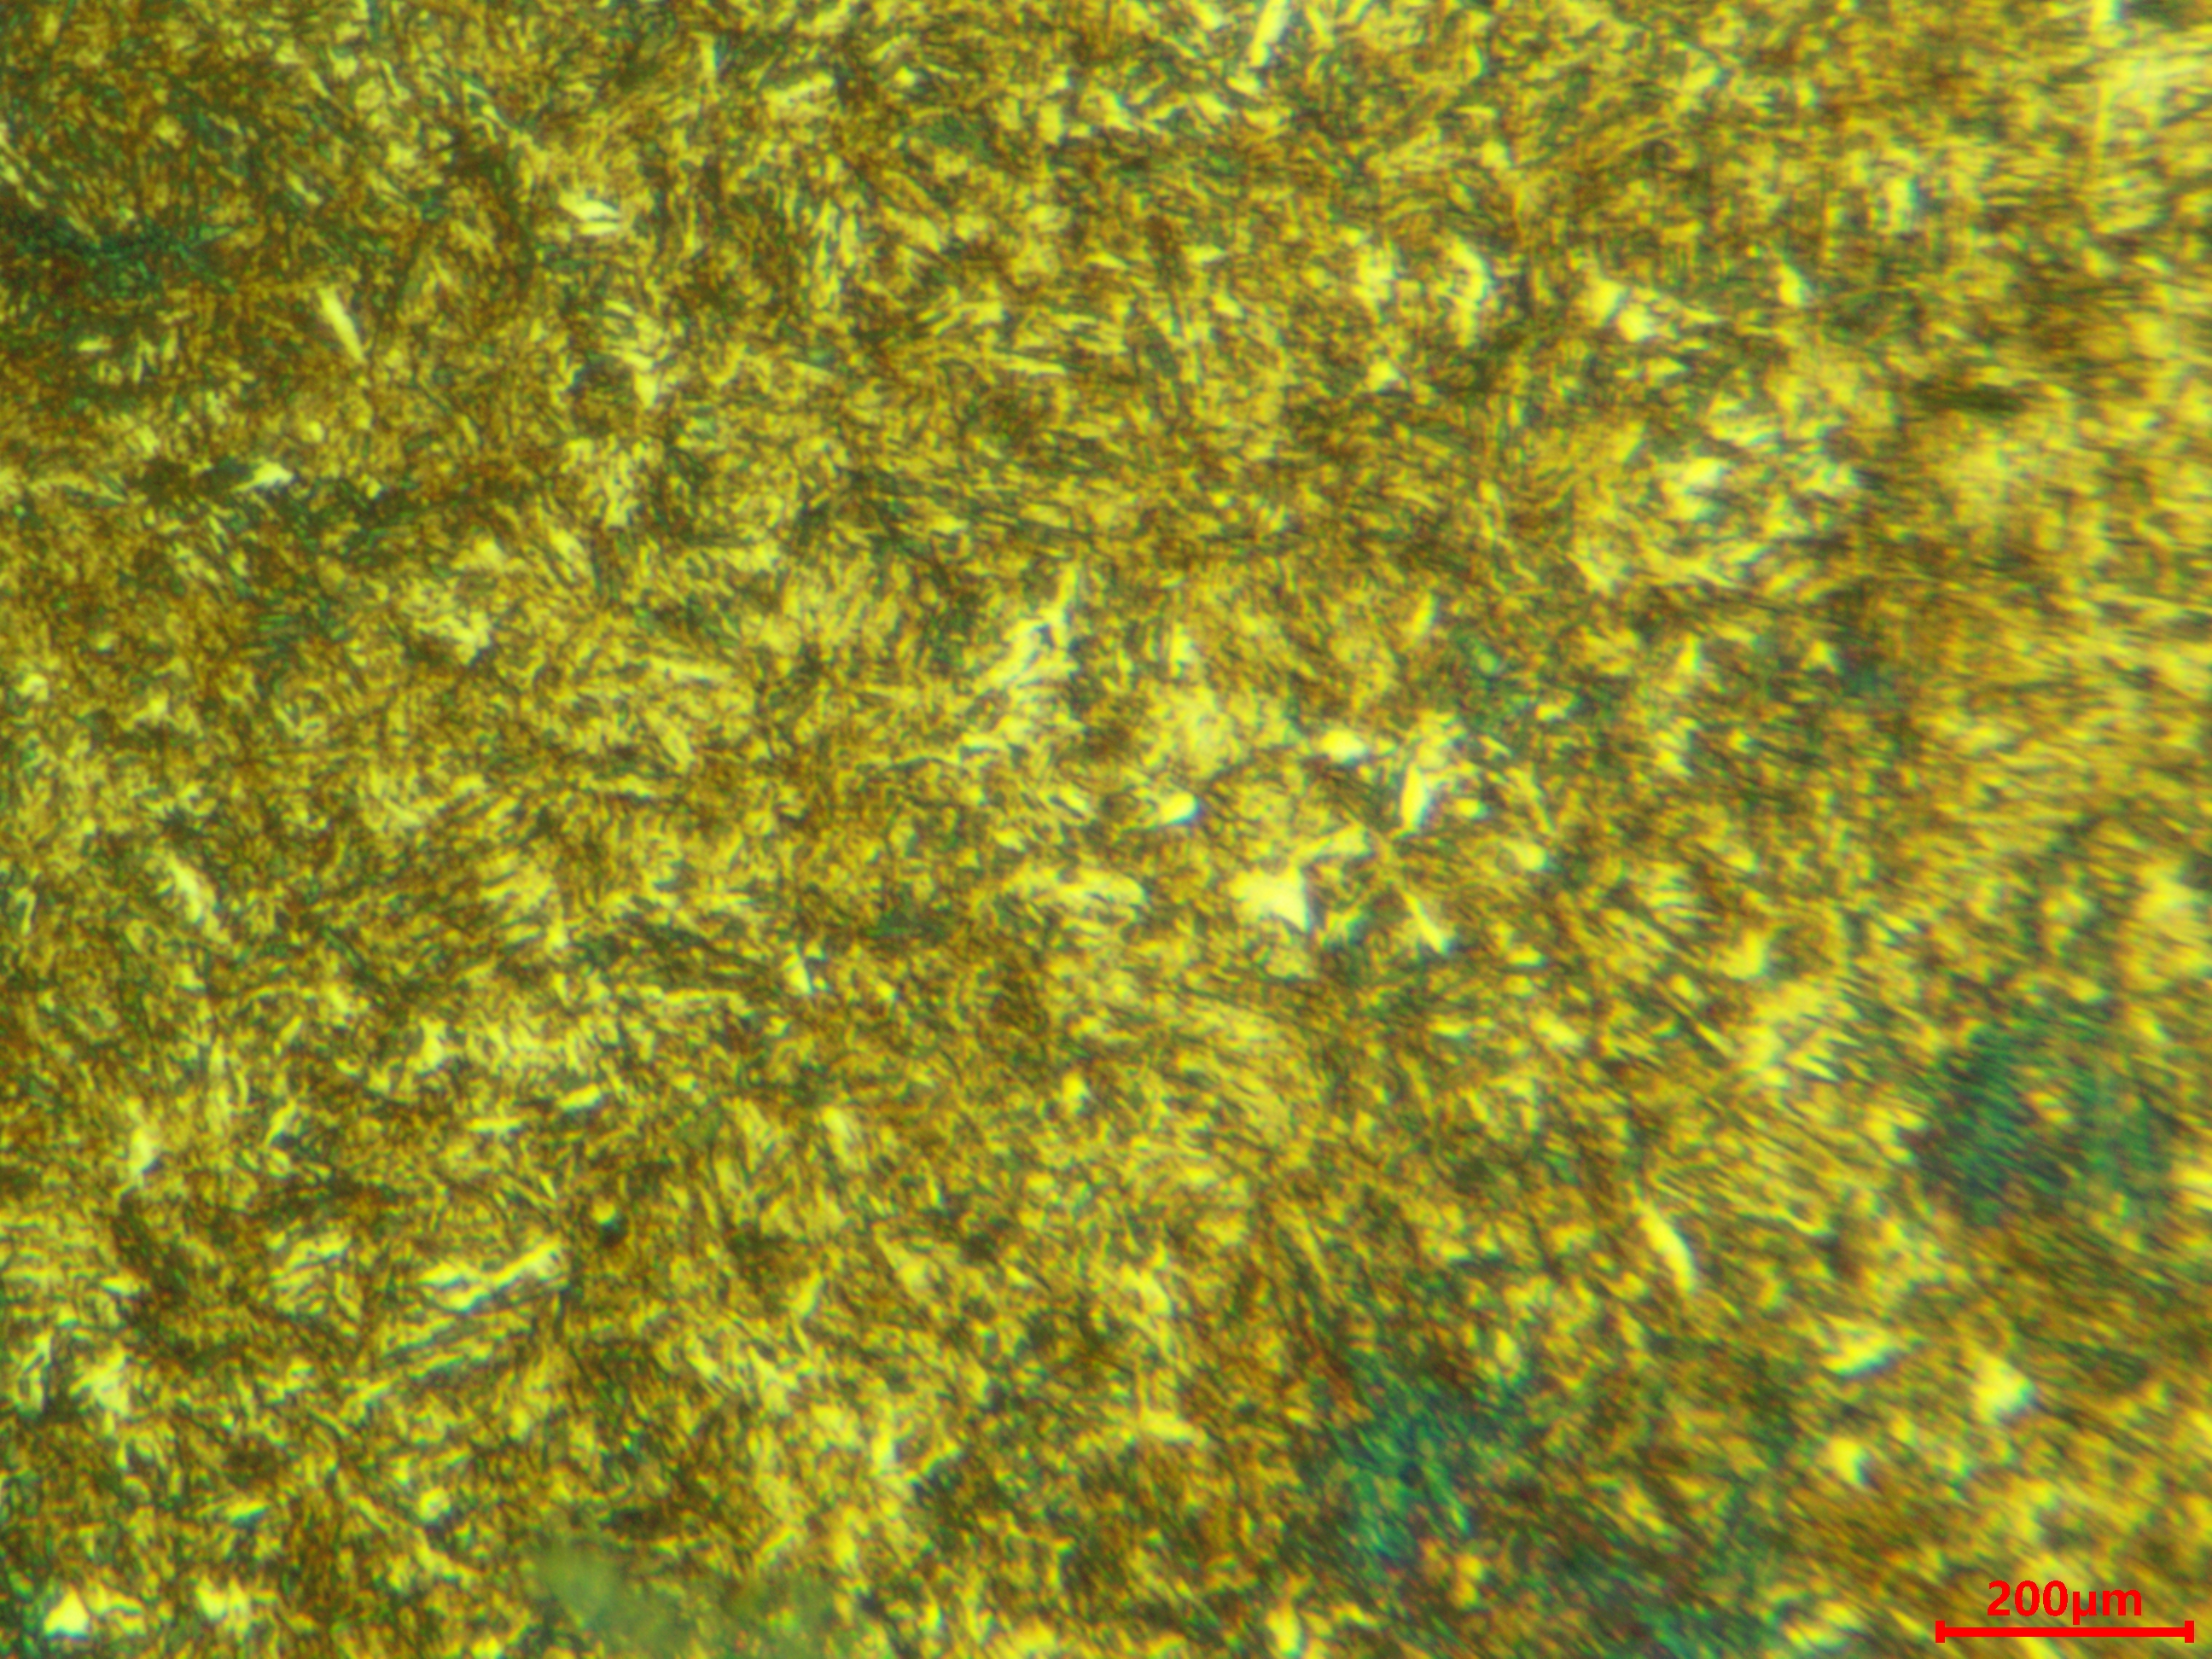
\includegraphics[width=60mm]{131.jpg}}
    \end{floatrow}

\end{figure}

分析:中碳钢淬火将得到细针状马氏体和板条状马氏体的混合组织;可以看出有许多细条状的马氏体集群,
不同集群之间的方向不一。同时这些细条状马氏体十分细小。
4).45钢水淬,400摄氏度回火
\begin{figure}[!ht]
    \begin{floatrow}
        \ffigbox[60mm]{\caption{445钢水淬,400摄氏度回火}}{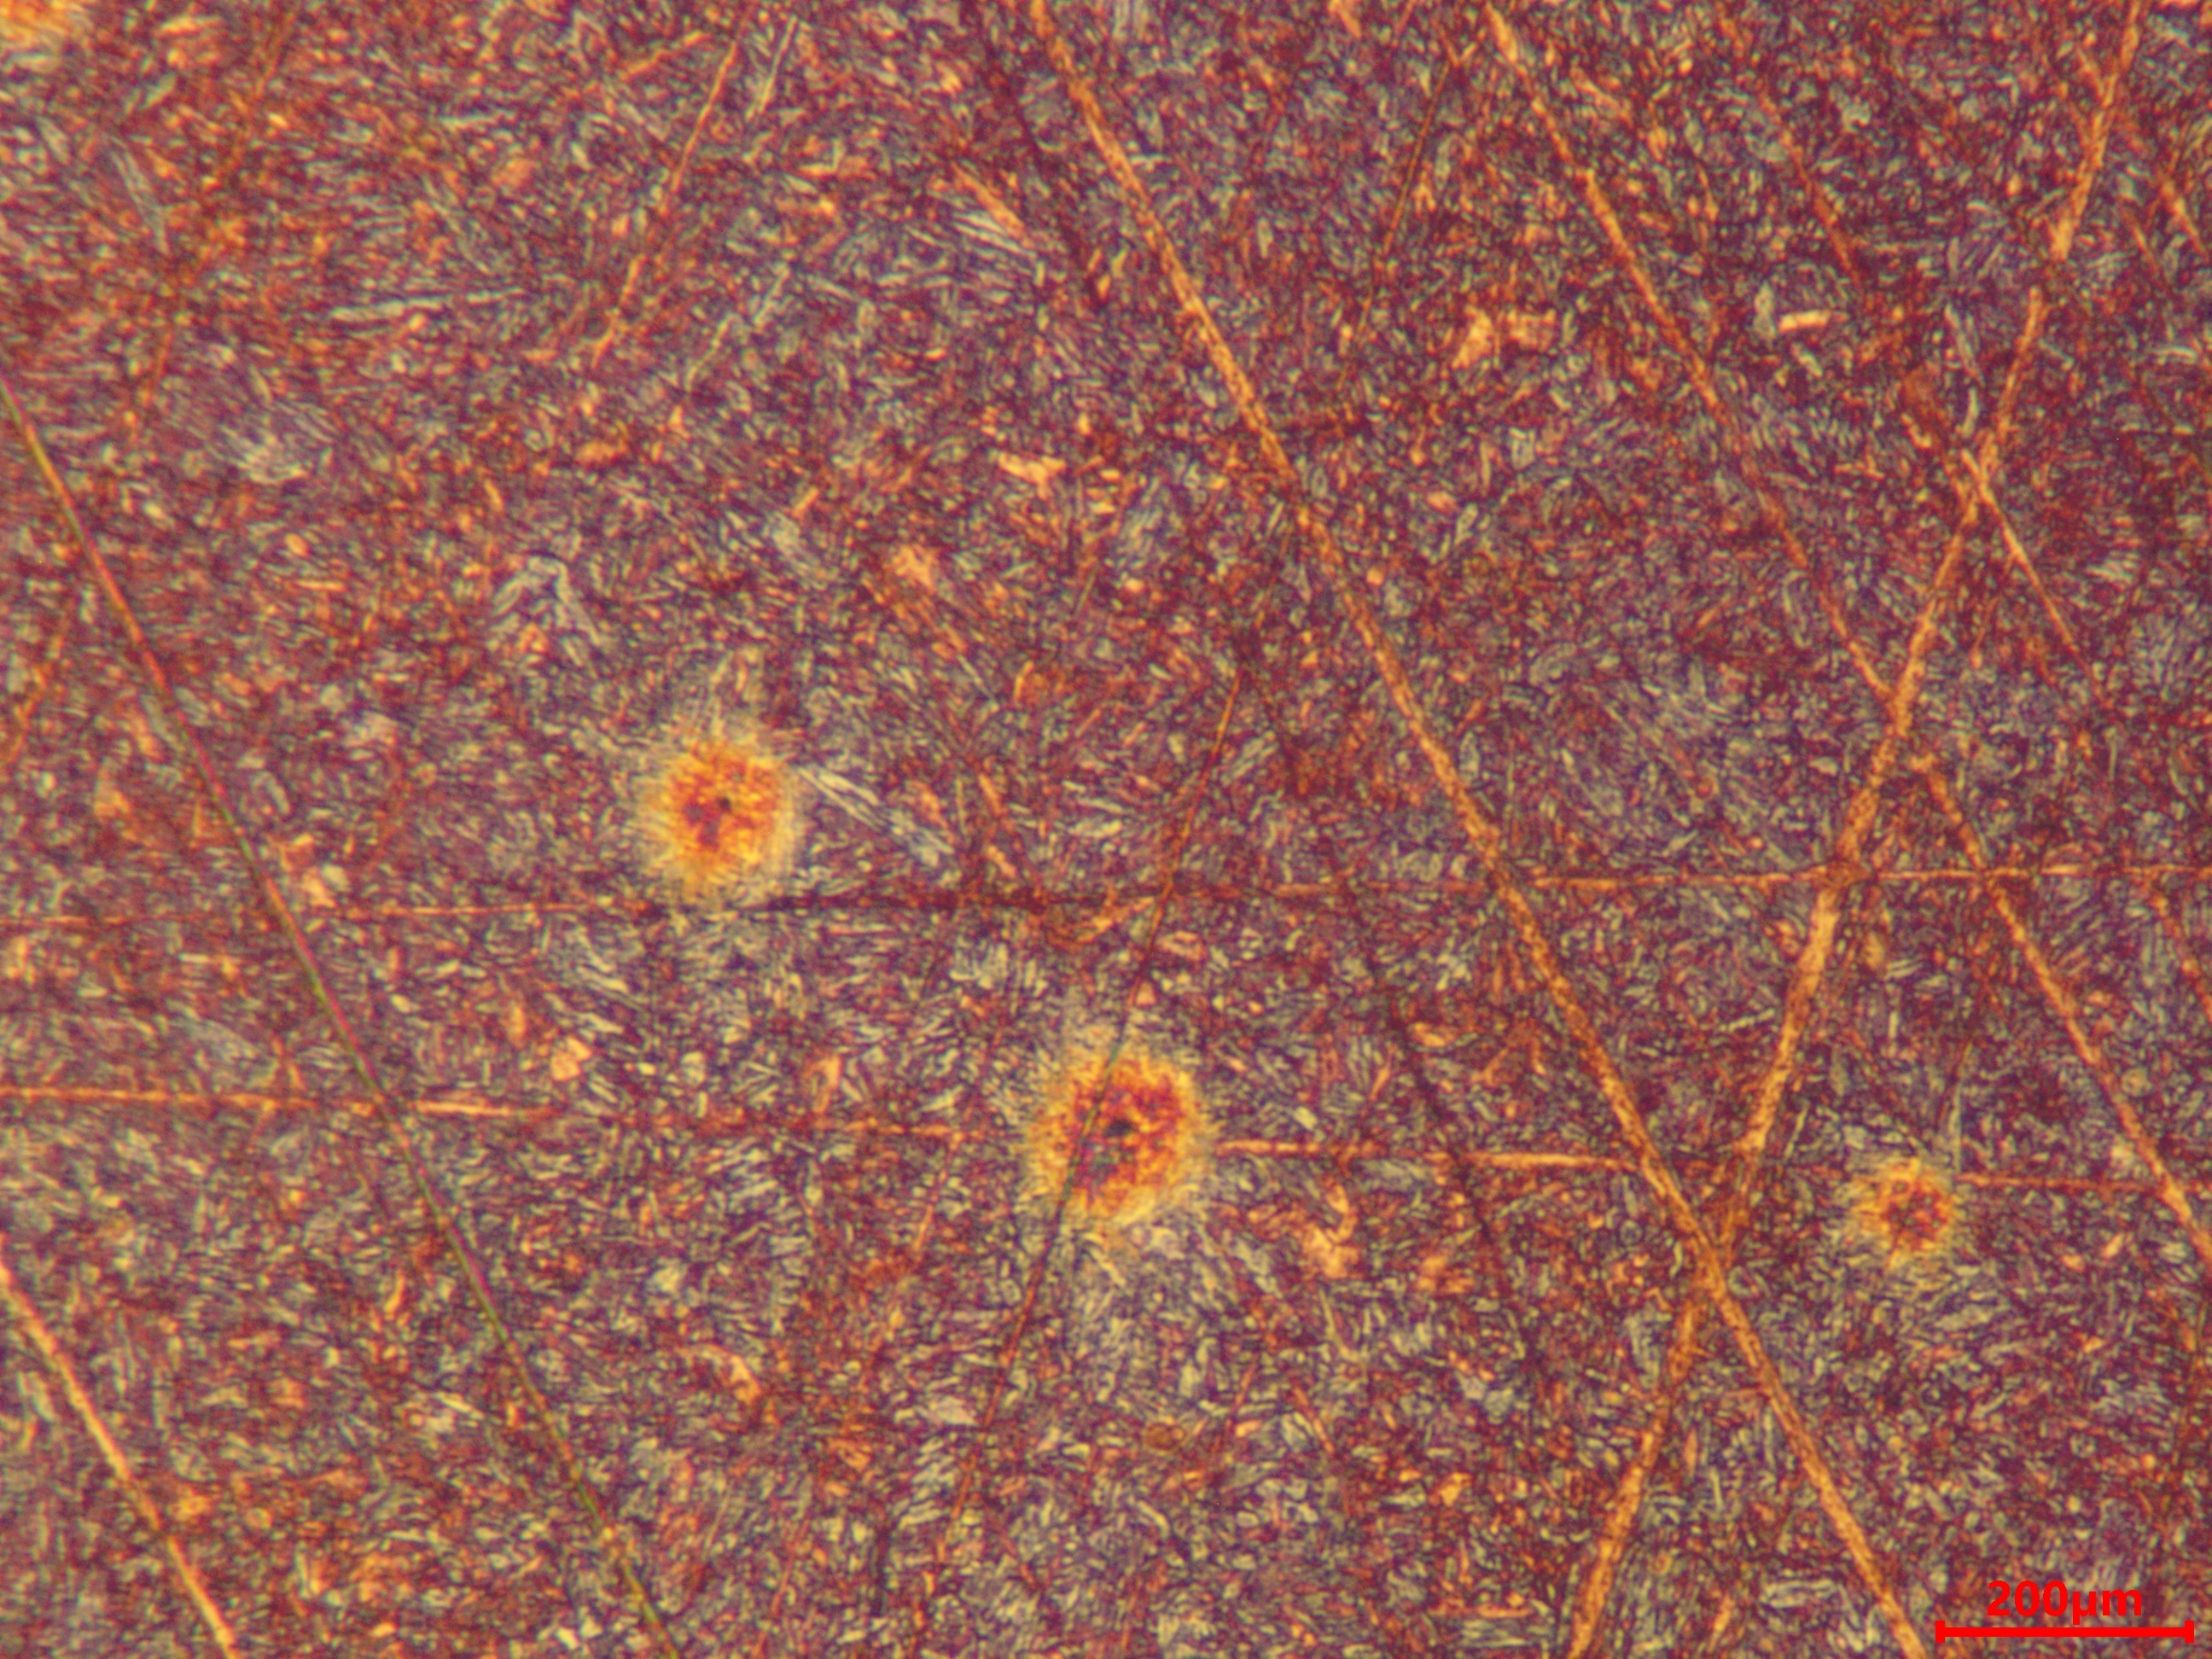
\includegraphics[width=60mm]{141.jpg}}
    \end{floatrow}

\end{figure}

分析:板条状马氏体较为明显,针状的马氏体比较难以发现,
在图中,片状的马氏体大小较小,针状的马氏体分布在片状马氏体旁边。铁素体基质上有粒状的渗碳体,呈现相对较深的颜色。

5).45钢水淬,600摄氏度回火
\begin{figure}[!ht]
    \begin{floatrow}
        \ffigbox[60mm]{\caption{45钢水淬,600摄氏度回火}}{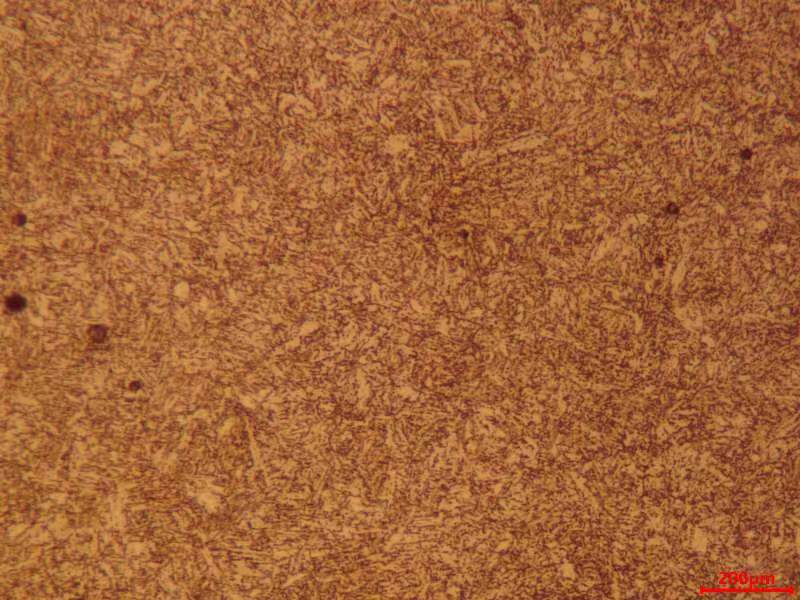
\includegraphics[width=60mm]{151.jpg}}
    \end{floatrow}

\end{figure}

分析:有颗粒状的渗碳体分散在基体中,马氏体更加细小,有球状的碳三铁析出,组织相对均匀,没有大块的奥氏体残余。

\section*{【思考题】}

淬火时的加热温度不同,冷却速度不同,其马氏体的形态有差异,中碳钢(碳含量界于0.25$\% \sim $0.6$\%$之间的非合金钢)经正常淬火后将得到细针
状马氏体和板条状马氏体的混合组织。油淬的钢其细针状马氏体较少,低温淬火则马氏体颗粒较大。
因而可以由此判断是温度不够还是淬火速度太慢。

\end{document}